\subsection{Apa itu SDLC?}
SDLC atau \emph{Systems Development Life Cycle}, atau  
dalam bahasa Indonesia disebut Siklus Hidup Pengembangan Sistem. SDLC adalah siklus yang 
digunakan dalam pembuatan atau pengembangan sistem informasi yang bertujuan untuk menyelesaikan
masalah secara efektif. Dalam pengertian lain, SDLC adalah tahapan kerja yang bertujuan untuk 
menghasilkan sistem berkualitas tinggi yang sesuai dengan keinginan pelanggan atau tujuan dibuatnya
sistem tersebut. SDLC menjadi kerangka yang berisi langkah-langkah yang harus dilakukan untuk 
memproses pengembangan suatu perangkat lunak. Sistem ini berisi rencana lengkap untuk mengembangkan, 
dan memelihara hasil produk software yang jadi.\cite{binus}

\subsection{Fungsi SDLC}
SDLC digunakan untuk membangun suatu sistem informasi agar dapat berjalan sesuai 
dengan apa yang diharapkan. SDLC (Systems Development Life Cycle) 
atau Systems Life Cycle, dalam rekayasa sistem dan rekayasa perangkat lunak, 
adalah proses pembuatan dan pengubahan sistem serta model dan metodologi yang digunakan untuk 
mengembangkan sistem-sistem tersebut. Konsep ini umumnya merujuk pada sistem komputer atau informasi. 
SDLC juga merupakan pola yang diambil untuk mengembangkan sistem perangkat lunak, yang terdiri dari 

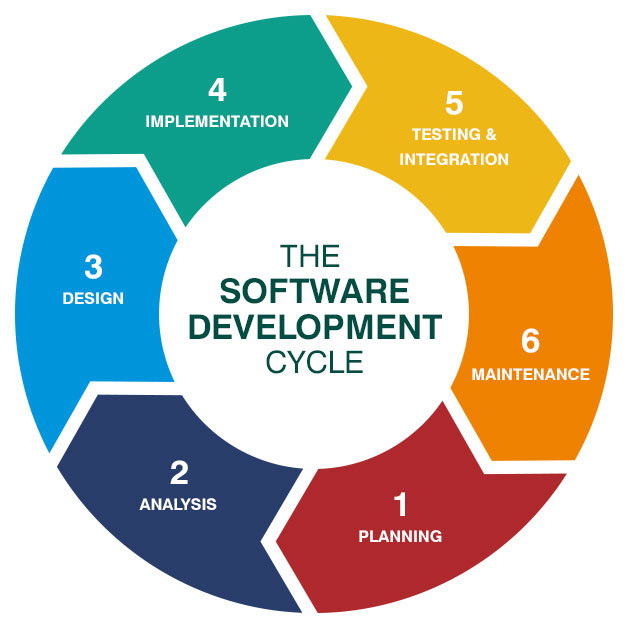
\includegraphics[width=0.4\textwidth]{images/sdlc-cycle.jpg}

\begin{enumerate}
    \item \emph{Planning} (rencana)
    \item \emph{Analysis} (analysis)
    \item \emph{Design} (design)
    \item \emph{Implementation} (penerapan)
    \item \emph{Testing} (uji coba)
    \item \emph{Maintenance} (pengelolaan)
\end{enumerate}

Dalam rekayasa perangkat lunak, konsep SDLC mendasari berbagai jenis metodologi 
pengembangan perangkat lunak. Metodologi-metodologi ini membentuk suatu kerangka kerja 
untuk perencanaan dan pengendalian pembuatan sistem informasi, yaitu proses pengembangan 
perangkat lunak. Terdapat 3 jenis metode siklus hidup sistem yang paling banyak digunakan, 
yakni: 

\begin{itemize}
    \item \emph{Traditional System Life Cycle}
    \item \emph{Life Cycle Using Prototyping}
    \item \emph{Object-oriented System Life Cycle}
\end{itemize}